\section{Method}
% \red{1. design kernel with cache update}

% \red{2. fuse kernels}

This section details the kernel implementation of MoDiff. We begin by refining the notation of MoDiff to clearly distinguish integer operations from floating-point operations. We then describe how the kernels are fused with cache updates in the U-Net architecture.

\subsection{Integer Arithmetic Formulation}
\paragraph{Diffusion Models.} sing Denoising Diffusion Probabilistic Models (DDPMs) as an example~\citep{ho2020denoising}, the forward process incrementally adds noise to the image at each step, gradually transforming the data distribution into a standard Gaussian distribution:
\begin{equation}
    q(\vx_t|\vx_{t-1})=N(\vx_t;\sqrt{1-\beta_t}\vx_{t-1},\beta_tI).
\end{equation}
Meanwhile, the reverse process progressively denoises the Gaussian distribution, reconstructing the original image distribution step by step with a denoising network:
\begin{equation}
    p_\theta(\vx_{t-1}|\vx_t)=N(\vx_{t-1};\mu_\theta(\vx_t,t),\sigma_t^2I),
\end{equation}
where \(\mu_\theta(\vx_t, t)\) is predicted by a neural network, while \(\sigma_t\) is typically set to \(\beta_t\). With this parametrization, the sampling process can be expressed as:
\begin{equation}
\label{eqn:diffusion}
    \vx_{t-1}=\frac{1}{\sqrt{1-\beta_t}}\left(\vx_t-\frac{\beta_t}{\sqrt{1-\bar{\alpha}_t}}\epsilon_\theta(\vx_t,t)\right)+\sigma_t\vz,
\end{equation}
where \(\bar{\alpha}_t = \prod_{i=1}^t (1 - \beta_t)\), and \(\epsilon_\theta(\vx_t, t)\) represents a U-Net that predicts the noise.

\begin{figure}
    \centering
    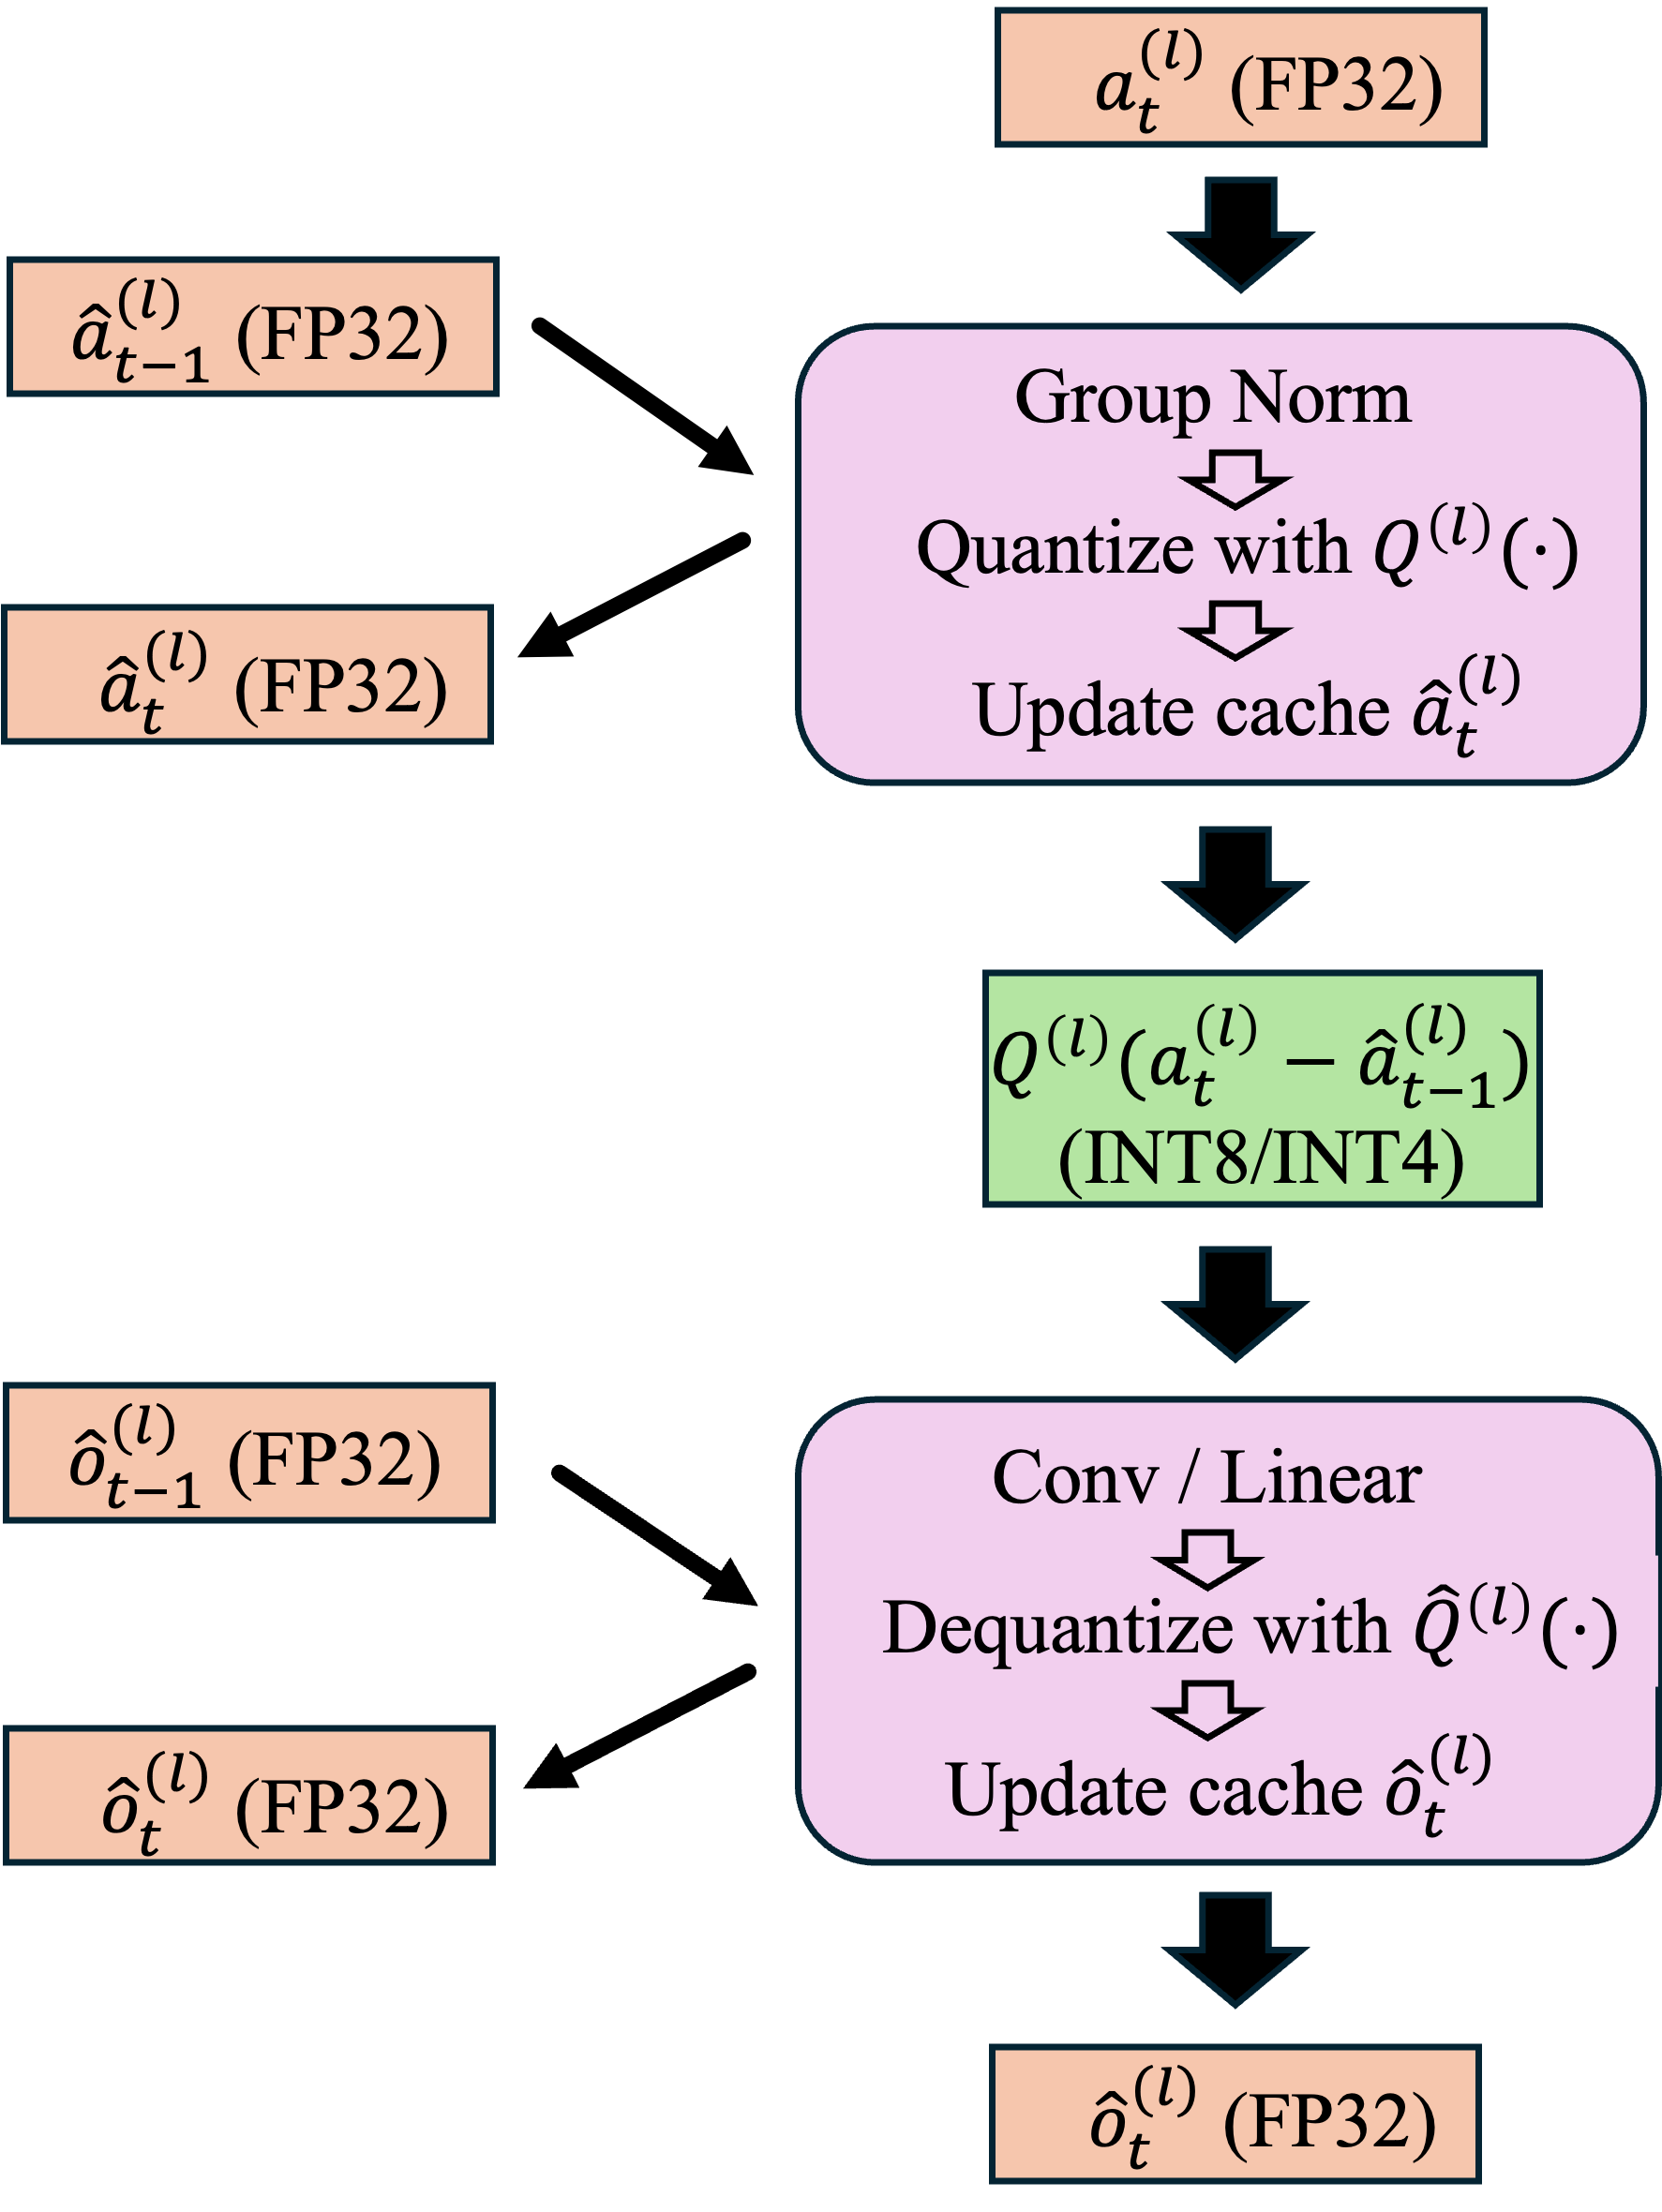
\includegraphics[width=0.72\linewidth]{figures/workflow.png}
    \caption{Kernel Design for MoDiff. The quantization operation and the update of $\hat\va_t^\ul$ are fused into the normalization layers, while the dequantization operation and the update of $\hat\vo_t^\ul$ are fused into the computational layers.}
\label{fig:kernel_design}
\end{figure}

\paragraph{Quantization.} Given FP input \(\mathbf{x}\), the quantizer $Q$ converts $\vx$ into an integer $\vx_\text{int}$ and the dequantizer $\hat Q$ converts it back to the floating-point numbers $\vx_\text{deq}$:
\begin{align}
    & \vx_{\text{int}} = Q(\vx) = \text{clamp}(\left\lfloor\frac{\vx}{s}\right\rceil + \vz; 0, 2^b-1), \\
    & \vx_\text{deq} = \hat Q(\vx_{\text{int}}) = s(\vx_{\text{int}}-\vz),
\end{align}
where \(b\) represents the quantization bitwidth, and \(\text{clamp}(\cdot)\) enforces value cut-offs between two integer bounds. The parameters \(s\) and \(\mathbf{z}\) correspond to the scale factor and zero point, respectively. For notational simplicity, we denote integer numbers with INT8/INT4 and floating-point numbers with FP32, where the numbers indicate the bitwidth.

\begin{table*}
    [bht]
    \centering
    \caption{Running time and DRAM transfer comparison on LSUN-Churches. DRAM transfers include weight, activation, output, cache read, and cache write. Speedup and DRAM transfer reduction are calculated against FP32.}
    \label{tab:pipeline_speedup} \resizebox{\linewidth}{!}{
    \begin{tabular}{lcc|crrrrrrl}
        \toprule & \multicolumn{2}{c|}{Runtime} & \multicolumn{7}{c}{DRAM Transfer (GB)} \\
        \cmidrule(lr){2-3}\cmidrule(lr){4-10} Mode & ms/Sample &  Speedup & Weight & Act & Output & Cache Rd & Cache Wr & Total & Ratio \\
        \midrule FP32 & 613.4 &  1.000$\times$ & 219.2 & 26.3 & 19.2 & 0.0 & 0.0& 264.6 & 100\% \\
        Baseline INT8 & 333.0  & 1.842$\times$& 66.2& 26.3 & 19.2 & 0.0 & 0.0 & 111.6 & 42.2\%  \\
        \textbf{MoDiff INT8 (Ours)}& \textbf{367.7} & \textbf{1.668$\times$} & 66.2& 26.3& 19.2& 51.6  & 36.9& \textbf{200.2} & \textbf{75.6\%}  \\
        Baseline INT4 & 306.2 & 2.003$\times$  & 42.6 & 26.3 & 19.2  & 0.0 & 0.0  & 88.0  & 33.2\%  \\
        \textbf{MoDiff INT4 (Ours)}& \textbf{340.9}& \textbf{1.800$\times$} & 42.6& 26.3& 19.2& 51.6& 36.9& \textbf{176.6} & \textbf{66.7\%}  \\
        \bottomrule
    \end{tabular}}
\end{table*}

\paragraph{Modulated Diffusion.} Modulated diffusion operates on linear operators in the denoising network, such as linear and convolutional layers. We take the $l$-th convolutional layer as an example. Its weight tensor is quantized, and for simplicity we denote the quantized weight as $\mathbf{w}^{(l)}_{\mathrm{int}}$. We use $*$ to denote FP convolution and $\circledast$ to denote INT convolution. At time step $t$, the input and output of the $l$-th convolutional layer are denoted by $\mathbf{a}_{t}^{(l)}$ and $\mathbf{o}_{t}^{(l)} = \vw_{\mathrm{int}}^\ul*\mathbf{a}_{t}^{(l)}$, respectively. Since the temporal difference $\mathbf{a}_{t}^{(l)} - \mathbf{a}_{t+1}^{(l)}$ is more amenable to quantization, modulated quantization applies the activation quantizer $Q^{(l)}$ to this difference and uses it to approximate $\mathbf{o}_{t}^{(l)}$ with $\hat{\mathbf{o}}_{t}^{(l)}$:
% Let $\mathcal{A}^{(l)}(\cdot)$ represent the $l$-th linear operator in the denoising network, such as linear or convolutional layers, where $l\in\{1,2,\ldots,L\}$. We use $\vw^{\ul}$ to denote the weight tensor of $\cA^{\ul}$, and $\vw^{\ul}_{\mathrm{int}}$ to denote its quantized counterpart $Q_{\vw}^{\ul}(\vw^{\ul})$ for simplicity. We denote the input and output for $\mathcal{A}^{(l)}(\cdot)$ at time step $t$ are $\mathbf{a}_{t}^{(l)}$ and $\vo_{t}^{(l)}=\cA^{(l)}(\va_{t}^{(l)})$, respectively. Because the temporal difference $\va_{t}^{\ul}- \va_{t+1}^{\ul}$ is more amenable to quantization, modulated quantization applies the activation quantizer $Q^{\ul}$ to this difference to approximate $\vo_{t}^{\ul}$ with $\hat\vo_{t}^{\ul}$. Take the 
% \begin{align}
%     \label{eqn:update_ahat}\hat\va_{t}^{(l)} & = Q^{\ul}(\va_{t}^{(l)}-\hat\va_{t+1}^{(l)}) + \hat\va_{t+1}^{(l)},           \\
%     \label{eqn:update_ohat}\hat\vo_{t}^{(l)} & = \cA^{(l)}(Q^{\ul}(\va_{t}^{(l)}-\hat\va_{t+1}^{(l)})) + \hat\vo_{t+1}^{(l)} \\
%     \label{eqn:otat}                         & =\cA^{(l)}(\hat\va_{t}^{\ul})\approx \vo_{t}^{\ul},
% \end{align}
\begin{align}
    \label{eqn:update_ahat}\hat\va_{t}^{(l)} & = \hat Q^\ul\left(Q^{\ul}(\va_{t}^{(l)}-\hat\va_{t+1}^{(l)})\right) + \hat\va_{t+1}^{(l)},           \\
    \label{eqn:update_ohat}\hat\vo_{t}^{(l)} & = \hat Q^\ul\left(\vw_\text{int}^{(l)}\circledast Q^{\ul}(\va_{t}^{(l)}-\hat\va_{t+1}^{(l)})\right) + \hat\vo_{t+1}^{(l)} \\
    \label{eqn:otat}                         & 
    % =\cA^{(l)}(\hat\va_{t}^{\ul})
    \approx \vw_{\mathrm{int}}^\ul*\va_t
    =\vo_{t}^{\ul},
\end{align}
where $t = T-1, \ldots, 1$, and $\hat{\va}_{t}^{\ul}$ serves as an intermediate variable to prevent error accumulation during generation by ensuring $\hat\vo_{t}^{\ul}=\cA(\hat\va_{t}^{\ul})$. The process is initialized with $\hat{\va}_{T}^{(l)}= \va_{T}^{(l)}$ and $\hat{\vo}_{T}^{(l)}= \vw^\ul_{\mathrm{int}}*\va_{T}^{(l)}$. The rewrite shows that all convolutional operations are performed using integer arithmetic. Although this approach is effective, introducing the caches $\hat\va_{t}^{\ul}$ and $\hat\vo_{t}^{\ul}$ necessitates accumulating historical computations, which poses challenges for kernel design in hardware acceleration.


% \begin{figure}[ht]
\centering
\begin{tikzpicture}[
font=\footnotesize,
node distance=0.45cm,
box/.style={draw, dashed, rounded corners, inner sep=6pt, align=center, fill=blue!8},
cache/.style={draw, rounded corners, fill=yellow!15, inner sep=4pt, align=center},
prec/.style={draw, rounded corners, inner sep=4pt, align=center},
arrow/.style={-{Stealth[length=0.8mm]}, line width=0.3pt}
]

% main pipeline
\node[prec, fill=green!10] (fp32in)
{$\va_t^{(l)}$ \\ \textbf{FP32}};

\node[box, below=of fp32in] (gn)
{GroupNorm \\ $Q^{(l)}$ \\ $\hat{\va}_t^{(l)}$ update \\ \textbf{FP32 → INT4/8}};

\node[prec, fill=orange!12, below=of gn] (int)
{$Q^{(l)}(\va_t^{(l)}-\hat{\va}_{t+1}^{(l)})$ \\ \textbf{INT4/8}};

\node[box, below=of int] (conv)
{Conv / Linear \\ $\hat Q$ \\ $\hat{\vo}_t^{(l)}$ update \\ \textbf{INT4/8 → FP32}};

\node[prec, fill=green!10, below=of conv] (fp32out)
{$\hat{\vo}_t^{(l)}$ \\ \textbf{FP32}};

% caches
\node[cache, left=0.9cm of gn] (acache)
{$\hat{\va}_{t+1}^{(l)}$ \\ \textbf{FP32 cache}};

\node[cache, right=0.9cm of gn] (acacheout)
{$\hat{\va}_t^{(l)}$ \\ \textbf{FP32 cache}};

\node[cache, left=0.9cm of conv] (ocache)
{$\hat{\vo}_{t+1}^{(l)}$ \\ \textbf{FP32 cache}};

\node[cache, right=0.9cm of conv] (ocacheout)
{$\hat{\vo}_t^{(l)}$ \\ \textbf{FP32 cache}};

% arrows main
\draw[arrow] (fp32in) -- (gn);
\draw[arrow] (gn) -- (int);
\draw[arrow] (int) -- (conv);
\draw[arrow] (conv) -- (fp32out);

% cache arrows
\draw[arrow] (acache) -- (gn);
\draw[arrow] (gn) -- (acacheout);

\draw[arrow] (ocache) -- (conv);
\draw[arrow] (conv) -- (ocacheout);

\end{tikzpicture}

\caption{The Kernel Design for MoDiff.}
\label{fig:kernel_design}
\end{figure}

\subsection{Kernel Fusion}

We design specialized kernel fusion methods for MoDiff to integrate cache accumulation into layer computation, thereby avoiding additional I/O overhead~\cite{cutlass,chen2018tvm,vasilache2018tensor}. Specifically, in the backbone, each convolutional layer is preceded by a GroupNorm layer. Therefore, we fuse the quantizer $Q$ and the update of the cache $\hat{\va}_t$ into the GroupNorm layer. We further fuse the dequantization operation $\hat Q$ and the update of the cache $\hat{\vo}_t$ into the post-accumulation stage of the convolutional layer. As shown in Figure~\ref{fig:kernel_design}, the GroupNorm layer takes the FP32 input $\va_t^{(l)}$ and the cache $\hat{\va}_{t+1}^{(l)}$ as inputs, and produces two outputs: the integer activation $Q^{(l)}\!\left(\va_t^{(l)}-\hat{\va}_{t+1}^{(l)}\right)$ for the subsequent forward computation, and the FP32 cache $\hat{\va}_t^{(l)}$ for the next diffusion step. The convolutional layer then takes the integer input $Q^{(l)}\!\left(\va_t^{(l)}-\hat{\va}_{t+1}^{(l)}\right)$ together with the cache $\hat{\vo}_{t+1}^{(l)}$, and outputs the FP32 activation $\hat{\vo}_t^{(l)}$ for forward propagation, which is also stored as the cache for the next step. Our design avoids additional I/O operations for the cache, improving the efficiency of the low-bit inference pipeline~\cite{chen2018tvm}.

% In this implementation, each quantized convolution is executed using two fused kernels. The first kernel manages activation-side preprocessing for the current timestep by computing the residual relative to the cached activation, estimating the quantization scale, quantizing the residual, and updating the activation cache in a single pass. The second kernel performs the CUTLASS tensor-core convolution on the quantized input and directly accumulates the result into the cached output feature map, eliminating the need for a separate post-convolution update step. These design choices reduce the overhead associated with layout conversion, synchronization, and allocation, thereby improving the efficiency of the low-bit inference pipeline. This design is illustrated in Fig.~\ref{fig:kernel_design}.


% We used PyTorch as the deep learning framework for our implementation. The code is based on the official MoDiff implementation available on GitHub. We made some modifications to the original code to adapt it to our specific use case.

% % % \red{main experiments: full pipeline inference, memory, write/read}

% To enhance performance, we incorporated the following optimizations:
% \begin{itemize}
%     \item {\textbf{CUTLASS}} Added CUTLASS(CUDA Templates for Linear Algebra Subroutines and Solvers) to optimize the performance of int8 and int4 convolutions.

%     \item {\textbf{Fused Kernels}} We implemented our kernel design as illustrated in Figure~\ref{fig:kernel_design} to enable efficient kernel fusion in conjunction with cache-update operations.

%     \item {\textbf{Other Optimizations}} We also introduced systematic buffer management and adopted a channel-last memory layout to enhance computational efficiency and overall performance further.
% \end{itemize}

% \begin{table*}
    [bht]
    \centering
    \caption{Running time and DRAM transfer comparison on LSUN-Churches. DRAM transfers include weight, activation, output, cache read, and cache write. Speedup and DRAM transfer reduction are calculated against FP32.}
    \label{tab:pipeline_speedup} \resizebox{\linewidth}{!}{
    \begin{tabular}{lcc|crrrrrrl}
        \toprule & \multicolumn{2}{c|}{Runtime} & \multicolumn{7}{c}{DRAM Transfer (GB)} \\
        \cmidrule(lr){2-3}\cmidrule(lr){4-10} Mode & ms/Sample &  Speedup & Weight & Act & Output & Cache Rd & Cache Wr & Total & Ratio \\
        \midrule FP32 & 613.4 &  1.000$\times$ & 219.2 & 26.3 & 19.2 & 0.0 & 0.0& 264.6 & 100\% \\
        Baseline INT8 & 333.0  & 1.842$\times$& 66.2& 26.3 & 19.2 & 0.0 & 0.0 & 111.6 & 42.2\%  \\
        \textbf{MoDiff INT8 (Ours)}& \textbf{367.7} & \textbf{1.668$\times$} & 66.2& 26.3& 19.2& 51.6  & 36.9& \textbf{200.2} & \textbf{75.6\%}  \\
        Baseline INT4 & 306.2 & 2.003$\times$  & 42.6 & 26.3 & 19.2  & 0.0 & 0.0  & 88.0  & 33.2\%  \\
        \textbf{MoDiff INT4 (Ours)}& \textbf{340.9}& \textbf{1.800$\times$} & 42.6& 26.3& 19.2& 51.6& 36.9& \textbf{176.6} & \textbf{66.7\%}  \\
        \bottomrule
    \end{tabular}}
\end{table*}
% \begin{figure}[ht]
    \centering
    \begin{minipage}[c]{0.48\linewidth}
        \centering
        \begin{tikzpicture}[
            font=\footnotesize,
            node distance=0.3cm,
            box/.style={
                draw,
                dashed,
                rounded corners,
                inner sep=4pt,
                align=center,
                fill=blue!8
            },
            arrow/.style={-{Stealth[length=1.6mm]}, thin}
        ]

            % Top
            \node[draw, rounded corners, fill=green!10, inner sep=3pt] (fp32in) {FP32};

            % First kernel
            \node[box, below=of fp32in] (k1) {GroupNorm\\[-0.2em] $\downarrow$\\[-0.2em] Quantize + $\hat{a}$ update};

            % Mid precision
            \node[draw, rounded corners, fill=orange!12, inner sep=3pt, below=of k1] (int) {Int8 / Int4};

            % Second kernel
            \node[box, below=of int] (k2) {Linear / Conv2d\\[-0.2em] $\downarrow$\\[-0.2em] Dequantize + $\hat{o}$ update};

            % Output
            \node[draw, rounded corners, fill=green!10, inner sep=3pt, below=of k2] (fp32out) {FP32};

            % Arrows
            \draw[arrow] (fp32in) -- (k1);
            \draw[arrow] (k1) -- (int);
            \draw[arrow] (int) -- (k2);
            \draw[arrow] (k2) -- (fp32out);

        \end{tikzpicture}
        \subcaption{Fused Kernel Design} 
        \label{fig:kernel_design}
    \end{minipage}
    \hfill
    \begin{minipage}[c]{0.48\linewidth}
        \centering
        % \rowcolors{2}{gray!10}{white}
        \begin{tabular}{c|c}
            % \rowcolor{gray!20}
            HyperParam / Env  & Value      \\
            GPU               & NVIDIA A40 \\
            Model             & LDM        \\
            Batch Size        & 32         \\
            Timesteps         & 200        \\
            Number of Samples & 128        \\
        \end{tabular}
        \subcaption{Benchmark Hyperparameter \& Environment} 
        \label{tab:bench_hyp_table}
    \end{minipage}
    \caption{Kernel Design and Benchmark Configuration}
    \label{fig:kernel_benchmark}
\end{figure}
% In this section, we describe our implementation of the MoDiff method and the optimizations we obtained.

% \begin{table*}
    [bht]
    \centering
    \caption{Running time and DRAM transfer comparison on LSUN-Churches. DRAM transfers include weight, activation, output, cache read, and cache write. Speedup and DRAM transfer reduction are calculated against FP32.}
    \label{tab:pipeline_speedup} \resizebox{\linewidth}{!}{
    \begin{tabular}{lcc|crrrrrrl}
        \toprule & \multicolumn{2}{c|}{Runtime} & \multicolumn{7}{c}{DRAM Transfer (GB)} \\
        \cmidrule(lr){2-3}\cmidrule(lr){4-10} Mode & ms/Sample &  Speedup & Weight & Act & Output & Cache Rd & Cache Wr & Total & Ratio \\
        \midrule FP32 & 613.4 &  1.000$\times$ & 219.2 & 26.3 & 19.2 & 0.0 & 0.0& 264.6 & 100\% \\
        Baseline INT8 & 333.0  & 1.842$\times$& 66.2& 26.3 & 19.2 & 0.0 & 0.0 & 111.6 & 42.2\%  \\
        \textbf{MoDiff INT8 (Ours)}& \textbf{367.7} & \textbf{1.668$\times$} & 66.2& 26.3& 19.2& 51.6  & 36.9& \textbf{200.2} & \textbf{75.6\%}  \\
        Baseline INT4 & 306.2 & 2.003$\times$  & 42.6 & 26.3 & 19.2  & 0.0 & 0.0  & 88.0  & 33.2\%  \\
        \textbf{MoDiff INT4 (Ours)}& \textbf{340.9}& \textbf{1.800$\times$} & 42.6& 26.3& 19.2& 51.6& 36.9& \textbf{176.6} & \textbf{66.7\%}  \\
        \bottomrule
    \end{tabular}}
\end{table*}
% % In this section, we describe our implementation of the MoDiff method and the optimizations we obtained.
% \subsection{Implementation Details}

% \begin{figure}[ht]
    \centering
    \begin{minipage}[c]{0.48\linewidth}
        \centering
        \begin{tikzpicture}[
            font=\footnotesize,
            node distance=0.3cm,
            box/.style={
                draw,
                dashed,
                rounded corners,
                inner sep=4pt,
                align=center,
                fill=blue!8
            },
            arrow/.style={-{Stealth[length=1.6mm]}, thin}
        ]

            % Top
            \node[draw, rounded corners, fill=green!10, inner sep=3pt] (fp32in) {FP32};

            % First kernel
            \node[box, below=of fp32in] (k1) {GroupNorm\\[-0.2em] $\downarrow$\\[-0.2em] Quantize + $\hat{a}$ update};

            % Mid precision
            \node[draw, rounded corners, fill=orange!12, inner sep=3pt, below=of k1] (int) {Int8 / Int4};

            % Second kernel
            \node[box, below=of int] (k2) {Linear / Conv2d\\[-0.2em] $\downarrow$\\[-0.2em] Dequantize + $\hat{o}$ update};

            % Output
            \node[draw, rounded corners, fill=green!10, inner sep=3pt, below=of k2] (fp32out) {FP32};

            % Arrows
            \draw[arrow] (fp32in) -- (k1);
            \draw[arrow] (k1) -- (int);
            \draw[arrow] (int) -- (k2);
            \draw[arrow] (k2) -- (fp32out);

        \end{tikzpicture}
        \subcaption{Fused Kernel Design} 
        \label{fig:kernel_design}
    \end{minipage}
    \hfill
    \begin{minipage}[c]{0.48\linewidth}
        \centering
        % \rowcolors{2}{gray!10}{white}
        \begin{tabular}{c|c}
            % \rowcolor{gray!20}
            HyperParam / Env  & Value      \\
            GPU               & NVIDIA A40 \\
            Model             & LDM        \\
            Batch Size        & 32         \\
            Timesteps         & 200        \\
            Number of Samples & 128        \\
        \end{tabular}
        \subcaption{Benchmark Hyperparameter \& Environment} 
        \label{tab:bench_hyp_table}
    \end{minipage}
    \caption{Kernel Design and Benchmark Configuration}
    \label{fig:kernel_benchmark}
\end{figure}
% We used PyTorch as the deep learning framework for our implementation. The code is based on the official MoDiff implementation available on GitHub. We made some modifications to the original code to adapt it to our specific use case.

% % % \red{main experiments: full pipeline inference, memory, write/read}

% To enhance performance, we incorporated the following optimizations:
% \begin{itemize}
%     \item {\textbf{CUTLASS}} Added CUTLASS(CUDA Templates for Linear Algebra Subroutines and Solvers) to optimize the performance of int8 and int4 convolutions.

%     \item {\textbf{Fused Kernels}} We implemented our kernel design as illustrated in Figure~\ref{fig:kernel_design} to enable efficient kernel fusion in conjunction with cache-update operations.

%     \item {\textbf{Other Optimizations}} We also introduced systematic buffer management and adopted a channel-last memory layout to enhance computational efficiency and overall performance further.
% \end{itemize}

% \subsection{Benchmarking and Performance}

% To evaluate the performance of our implementation, we conducted benchmarking experiments. We ran the experiments on a machine equipped with an NVIDIA A40 GPU, using the hyperparameters listed in Table \ref{tab:bench_hyp_table}.

% We compared the performance of our implementation with the FP32 generation, the int8-quantized generation without MoDiff, and the int4-quantized generation without MoDiff. The result of our benchmarking is shown in Table \ref{tab:pipeline_speedup} and visualized in Figure \ref{fig:plot_01_pipeline_speedup}. Through this benchmark, we demonstrated that our implementation achieves significant reductions in both computational and memory I/O costs. Through this benchmark, we demonstrated that our implementation achieves significant reductions in both computational and memory I/O costs.

% \begin{figure*}[t]
    \centering
    \begin{minipage}[c]{0.25\linewidth}
        \centering
        \begin{tabular}{lccc}
            \toprule \textbf{Mode} & \textbf{FID Score} & \textbf{Samples} \\
            \midrule FP32          & 5.73               & 50000            \\
            INT8                   & 5.85               & 50000            \\
            INT4                   & 14.80              & 50000            \\
            \bottomrule
        \end{tabular}
        \subcaption{FID Evaluation Results} \label{tab:fid_eval}
    \end{minipage}
    \hfill
    \begin{minipage}[c]{0.68\linewidth}
        \centering
        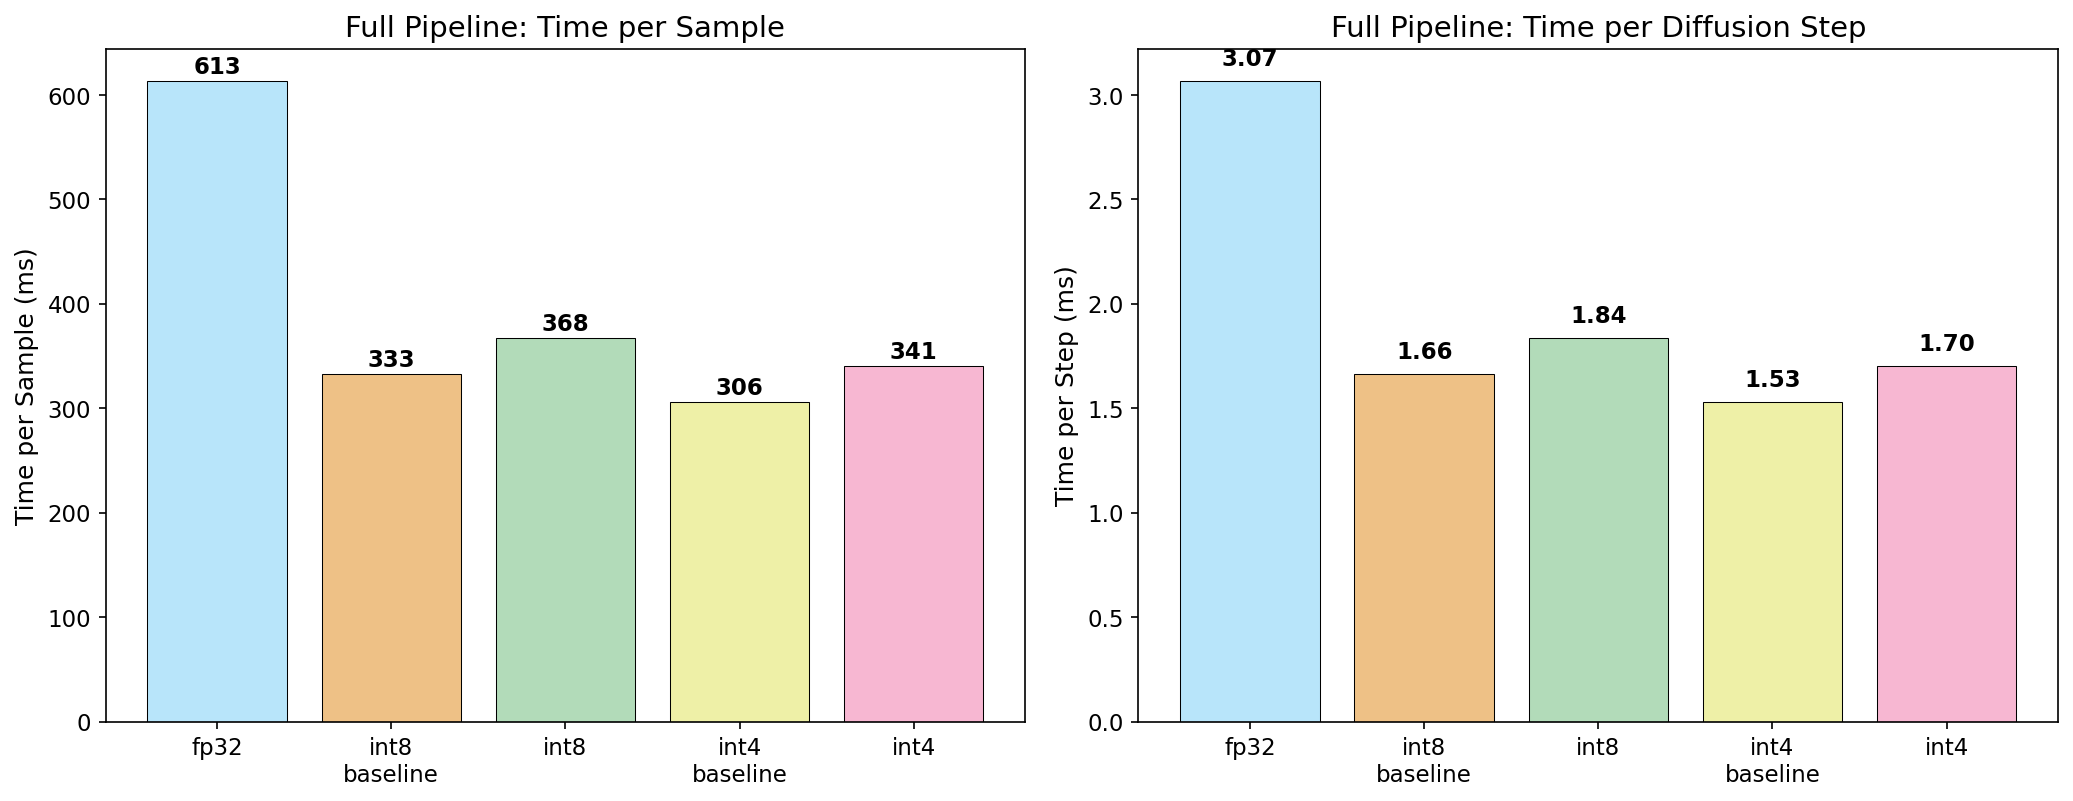
\includegraphics[width=\linewidth]{figures/plot_01_pipeline_speedup.png}
        \subcaption{Benchmark Results for Model Performance Optimization} \label{fig:plot_01_pipeline_speedup}
    \end{minipage}
    \caption{Performance and Quality Evaluation}
    \label{fig:plot_fid_combined}
\end{figure*}

% As shown in the results, our implementation of MoDiff with int8 quantization and int4 quantization achieved significant speedups compared to the FP32 generation. The int8-quantized generation with MoDiff achieved a speedup of 1.668x, while the int4-quantized generation with MoDiff achieved a speedup of 1.800x compared to the FP32 generation. These results demonstrate the effectiveness of our optimizations and the potential of MoDiff for accelerating deep learning models.

% To demonstrate that our implementation meets the quality expectations of the original MoDiff, we also evaluated the quality of the generated images using FID (Fréchet Inception Distance). The FID scores for the FP32 generation, int8-quantized generation with MoDiff, and int4-quantized generation with MoDiff are shown in Figure \ref{fig:plot_fid_combined}.